%!TEX root = Progetto.tex
\section{Codifica Sql e Testing} % (fold)
\label{sec:codifica_sql_e_testing}

Di seguito è riportata la definizione dello schema in linguaggio sql così come è implementato nel dump. Si allegano, per ogni tabella, degli screenshot dal terminale.

Il DBMS utilizzato (MySQL 5) nativamente non supporta la definizione di vincoli d'integrità personalizzabili. Per ovviare a questa limitazione, nell'implementazione completa dello schema (riportata nel dump) si è fatto un larghissimo uso di trigger che implementano la logica dei vincoli.

	\subsection{Definizione dello schema e screenshot successivi all'inserimento di dati}
		% Cliente

		\pagebreak
	\subsection{Codifica delle operazioni}
		Di seguito vengono riportate le implementazioni delle operazioni effettuabili sulla base di dati. La loro organizzazione non è lineare come l'elenco presentato in fase progettuale, ma rispecchia quelli che sono i reali casi d'uso.

		\subsubsection{Inserimento di un nuovo cliente}
			A tale inserimento corrisponde sempre l'inserimento e l'associazione di una nuova autovettura e di almeno un recapito.
				\begin{lstlisting}
/** Cliente non dotato di partita iva */
INSERT INTO Cliente (CF_PIVA, Nome, Cognome, Citta, 
	Via, Civico, CAP, NDocId) 
VALUES (...);

/** Cliente dotato di partita iva */
INSERT INTO Cliente (CF_PIVA, RagioneSociale, Citta, 
	Via, Civico, CAP) 
VALUES (...);

/** Inserimento dell'autovettura */
INSERT INTO Autovettura (Targa, Telaio, Marca, Modello, 
	Cilindrata, AnnoImmatricolazione, UltimoCollaudo, 
	UltimaRevisione, Cliente) 
VALUES (..., <CF_PIVA del cliente appena inserito>);

/** Inserimento di un recapito */
INSERT INTO Recapito (Recapito, Tipo)
VALUES (...);

/** Associazione di un recapito inserito al cliente */
INSERT INTO RubricaCliente (Recapito, Cliente)
VALUES (<Codice del recapito>, <CF_PIVA del cliente>);
				\end{lstlisting}

        \begin{figure}[H]
          \centering
          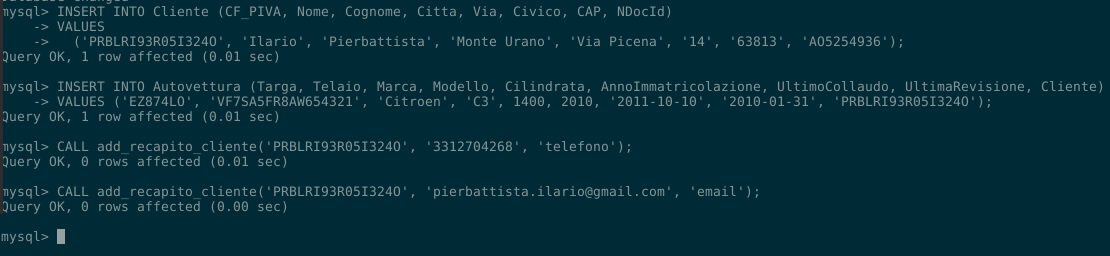
\includegraphics[width=15cm]{images/screenshots/nuovo_cliente.png}
        \end{figure}

        \begin{figure}[H]
          \centering
          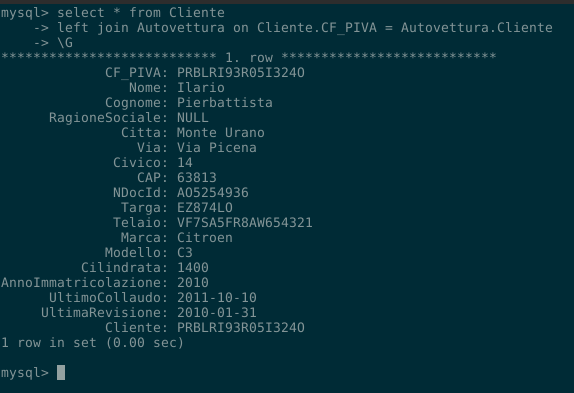
\includegraphics[width=9cm]{images/screenshots/show_cliente_autovettura.png}
        \end{figure}

			L'aggiunta di un recapito ad un cliente è un'operazione molto frequente. Per questo è stata creata una procedura che si occupa dell'inserimento e dell'associazione dello stesso:
				\begin{lstlisting}
CREATE PROCEDURE add_recapito_cliente(
  IN cf_piva  VARCHAR(16),
     recapito VARCHAR(200),
     tipo     ENUM('telefono',
                   'fax',
                   'tel_fax',
                   'sito_web',
                   'email')
)
  BEGIN
    DECLARE EXIT HANDLER FOR SQLEXCEPTION
    BEGIN
      ROLLBACK;
      /* La procedura throw_error si occupa di lanciare 
       * un segnale d'errore con codice 45000
       * e con il messaggio specificato come argomento
       */
      CALL throw_error('Recapito già registrato');
    END;
    START TRANSACTION;
    INSERT INTO Recapito (Recapito, Tipo) VALUES (recapito, tipo);
    SELECT LAST_INSERT_ID()
    INTO @last_id;
    INSERT INTO RubricaCliente (Recapito, Cliente) VALUES (@last_id, cf_piva);
    COMMIT;
  END;;
				\end{lstlisting}

        \begin{figure}[H]
          \centering
          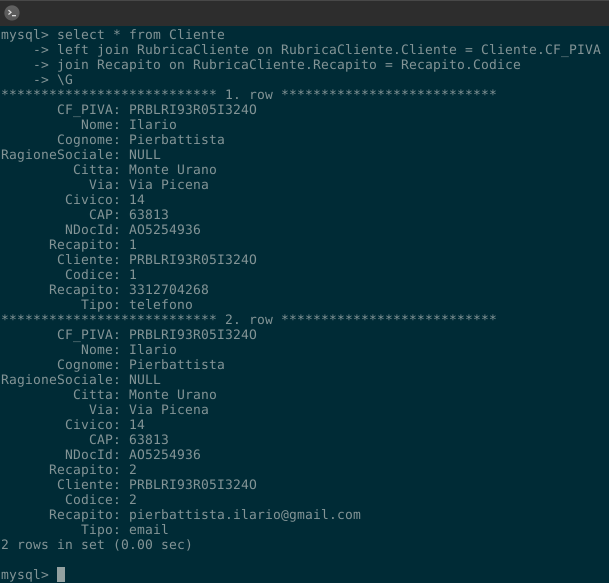
\includegraphics[width=9cm]{images/screenshots/show_cliente_rubrica.png}
        \end{figure}


			\subsubsection{Inserimento di un nuovo fornitore}
				All'inserimento di un nuovo fornitore corrisponde l'inserimento dei relativi recapiti.
				\begin{lstlisting}
/** Inserimento del fornitore */
INSERT INTO Fornitore (PIVA, RagioneSociale, TempiConsegna,
	ModPagamento, IBAN, Citta, Via, Civico, CAP) 
VALUES (...);

/** Associazione di un recapito inserito al fornitore
	(L'operazione di inserimento di un nuovo recapito
	è identica a quella presentata nel caso d'uso 
	precedente) */
INSERT INTO RubricaFornitore (Recapito, Fornitore)
VALUES (<Codice del recapito>, <PIVA del fornitore>);
				\end{lstlisting}

				Come nel caso precedente, anche per il fornitore esiste una procedura per l'aggiunta e l'associazione di un recapito.
				Gli inserimenti diventano molto più compatti:

				\begin{lstlisting}
CALL add_recapito_fornitore(<PIV del fornitore>,
	<recapito>, <tipo del recapito>);
				\end{lstlisting}

        Vista la semplicità di queste operazioni, non crediamo sia necessario allegare degli screenshot che ne testimonino la corretta esecuzione.


			\subsubsection{Inserimento di un nuovo operatore}
				Anche in questo caso bisognerà aggiungere uno o più recapiti a quest'ultimo. Presentiamo inoltre anche l'istruzione per inserire un nuovo turno di lavoro.
				\begin{lstlisting}
/** Inserimento di un operatore con stipendio fisso */
INSERT INTO Operatore (CF, Nome, Cognome, Citta, Via, 
	Civico, CAP, DataNasc, ComuneNasc, ProvinciaNasc, 
	Stipendio, ModRiscossione, IBAN)
VALUES (...);

/** Inserimento di un operatore con retribuzione
	oraria */
INSERT INTO Operatore (CF, Nome, Cognome, Citta, Via,
	Civico, CAP, DataNasc, ComuneNasc, ProvinciaNasc, 
	RetribuzioneH, ModRiscossione, IBAN)
VALUES (...);

/** Inserimento di un nuovo turno di lavoro */
INSERT INTO Turno (Operatore, Data, OraInizio, OraFine)
VALUES (<CF dell'operatore>, ...);

/** Aggiunta di un recapito */
CALL add_recapito_operatore(<CF dell'operatore>, <recapito>, 
	<tipo di recapito>)
				\end{lstlisting}

        Considerata la semplicità e l'analogia con i casi precedenti, non crediamo sia necessario allegare degli screenshot.


			\subsubsection{Inserimento di un nuovo componente}
				\begin{lstlisting}
INSERT INTO Componente (Nome, QuantitaMin, Validita, 
	PrezzoVendita) 
VALUES (...);
				\end{lstlisting}


			\subsubsection{Inserimento di un nuovo ordine}
				Questa operazione si articola in più parti: innanzi tutto bisogna creare una nuova istanza nella relazione \emph{Ordine}, quindi creare le istanze relative alle forniture dell'ordine.

				\begin{lstlisting}
/** Creazione del nuovo ordine */
INSERT INTO Ordine (DataEmissione, Fornitore, Imponibile) 
VALUES (...);

/** Creazione delle nuove forniture */
INSERT INTO Fornitura (Quantita, Componente, 
	Ordine, PrezzoUnitario)
VALUES (...), ..., (...);
				\end{lstlisting}

				In fase di creazione dell'ordine, inoltre, non è strettamente necessario inserirne l'imponibile. Lo si può calcolare in un secondo momento in base alle forniture associategli:

				\begin{lstlisting}
/** Aggiornamento dell'imponibile dell'ordine in base
 *  alle forniture associate allo stesso.
 *  Utilizzo della funzione calc_imponibile_ordine
 */
UPDATE Ordine
SET Imponibile = calc_imponibile_ordine(<Codice ordine>)
WHERE Ordine.Codice = <Codice ordine>;
				\end{lstlisting}

				Di seguito il corpo della funzione che automatizza il calcolo dell'attributo imponibile.

				\begin{lstlisting}
/** Implementazione di calc_imponibile_ordine
 *  Il primo parametro è il codice dell'ordine 
 */
CREATE FUNCTION calc_imponibile_ordine(ordine INTEGER)
  RETURNS DECIMAL(10, 2)
  BEGIN
    DECLARE result DECIMAL(10, 2);
    SELECT SUM(Fornitura.PrezzoUnitario * Fornitura.Quantita)
    FROM Ordine
      JOIN Fornitura ON Ordine.Codice = Fornitura.Ordine
    WHERE Ordine.Codice = ordine
    INTO result;
    RETURN result;
  END;;
				\end{lstlisting}

				Al pagamento dell'ordine, sarà necessario inserire una nuova transazione per registrare il pagamento al fornitore;

				\begin{lstlisting}
INSERT INTO Transazione (Quota, Data) VALUES (...);
UPDATE Ordine
SET Ordine.Versamento = <Codice della transazione>,
WHERE Ordine.Codice = <Codice dell'ordine>;
				\end{lstlisting}

				Ricordiamo che l'ammontare di tale transazione corrisponde all'imponibile dell'ordine cui vengono sommate le imposte ed altre somme eventuali. Per calcolare tale valore velocemente, si può utilizzare la funzione \emph{calc\_transazione\_ordine}:

				\begin{lstlisting}
/** Inserimento di una nuova transazione
 *  calcolando in modo automatico la quota 
 */
INSERT INTO Transazione (Quota, Data)
VALUES (calc_transazione_ordine(<Codice ordine>, 0), <Data>);

/**
 * Corpo della funzione calc_transazione_ordine
 * ordine: Codice dell'ordine di cui calcolare
 * 		il totale
 * plus: Somma aggiuntiva da aggiungere eventualmente
 * 		al risultato finale.
 */
CREATE FUNCTION calc_transazione_ordine(ordine INTEGER, plus REAL)
  RETURNS DECIMAL(10, 2)
  BEGIN
    DECLARE result DECIMAL(10, 2);
    SELECT Imponibile * (-(1 + IVA()))
    FROM Ordine
    WHERE Codice = ordine
    INTO result;
    RETURN result + plus;
  END;;
				\end{lstlisting}

				Infine, alla consegna dell'ordine da parte del fornitore, bisogna registrare la data di consegna ed inserire le nuove forniture nel magazzino.

				\begin{lstlisting}
/** Per ogni fornitura dell'ordine */
INSERT INTO Magazzino (Componente, Fornitura, Quantita)
VALUES (...);

/** Registrazione della data di consegna */
UPDATE Ordine
SET Ordine.DataConsegna = <Data di Consegna>
WHERE Ordine.Codice = <Codice dell'ordine>;
				\end{lstlisting}

				Infine anche per l'inserimento delle nuove forniture in magazzino abbiamo preparato una procedura che automatizza tale processo.

				\begin{lstlisting}
CALL registra_ordine_magazzino(<Codice dell'ordine>);

/** Corpo della funzione registra_ordine_magazzino
 * ordine: Codice dell'ordine di cui inserire le
 * 		forniture in magazzino 
 */
CREATE PROCEDURE registra_ordine_magazzino(IN ordine INTEGER)
  BEGIN
    DECLARE done BOOLEAN DEFAULT FALSE;
    DECLARE componente_id INT;
    DECLARE fornitura_id INT;
    DECLARE quantita INT;
    DECLARE cur CURSOR FOR
      SELECT
        Fornitura.Codice,
        Fornitura.Componente,
        Fornitura.Quantita
      FROM Fornitura
      WHERE Fornitura.Ordine = ordine;
    DECLARE CONTINUE HANDLER FOR NOT FOUND SET done = 1;
    DECLARE EXIT HANDLER FOR SQLEXCEPTION
    BEGIN
      ROLLBACK;
      CALL throw_error('Errore nell''inserimento dell''ordine in magazzino');
    END;
    START TRANSACTION;
    OPEN cur;
    REPEAT
      FETCH cur
      INTO fornitura_id, componente_id, quantita;
      IF NOT done
      THEN
        INSERT INTO Magazzino (Componente, Fornitura, Quantita)
        VALUES (componente_id, fornitura_id, quantita);
      END IF;
    UNTIL done END REPEAT;
    CLOSE cur;
    COMMIT;
  END;;
				\end{lstlisting}


			\subsubsection{Inserimento di un nuovo preventivo}

				\begin{lstlisting}
/** Inserimento di un nuovo preventivo */
INSERT INTO Preventivo (DataEmissione, DataInizio, Categoria,
	Sintomi, SisAlimentazione, TempoStimato, CostoComponenti, 
	Manodopera, ServAggiuntivi, Autovettura)
VALUES (...);

/** Inserimento dei componenti previsti */
INSERT INTO Previsione (Componente, Preventivo, 
	Ubicazione, Quantita)
VALUES (...), ..., (...);
				\end{lstlisting}

				Il costo dei componenti previsti dal preventivo può essere calcolato automaticamente alla fine dell'inserimento dei componenti previsti nella tabella \emph{Previsione}. Per far ciò abbiamo implementato una funzione chiamata \emph{calc\_costo\_componenti\_preventivo}.
				Inoltre, alla stipulazione di un preventivo, si può lasciare un acconto che viene regolarmente registrato.

				\begin{lstlisting}
/** Calcolo automatico del costo dei componenti */
UPDATE Preventivo 
SET CostoComponenti = calc_costo_componenti_preventivo(<Codice preventivo>)
WHERE Preventivo.Codice = <Codice preventivo>;

/** Inserimento di un acconto */
INSERT INTO Transazione (Quota, Data)
VALUES (...);
UPDATE Preventivo
SET Acconto       = <Codice della Transazione>,
WHERE Preventivo.Codice = <Codice del preventivo>;

/** Corpo della funzione calc_costo_componenti_preventivo
 *  preventivo: Codice del preventivo di cui calcolare il 
 * 			costo dei componenti
 */
CREATE FUNCTION calc_costo_componenti_preventivo(preventivo INTEGER)
  RETURNS DECIMAL(10, 2)
  BEGIN
    DECLARE result DECIMAL(10, 2);
    SELECT SUM(Previsione.PrezzoUnitario * Previsione.Quantita)
    FROM Preventivo
      LEFT JOIN Previsione ON Preventivo.Codice = Previsione.Preventivo
    WHERE Preventivo.Codice = preventivo
    INTO result;
    RETURN result;
  END;;
				\end{lstlisting}


      \subsubsection{Inserimento di una nuova prestazione}
        Questo caso d'uso è abbastanza macchinoso. Per la prestazione inserita bisogna specificare quali componenti sono stati utilizzati e di quali forniture, quali operatori l'hanno eseguita, quindi bisogna stilare una nuova fattura. Bisogna inoltre aggiornare il magazzino, decrementando le quantità dei componenti utilizzati.
        Stilata la fattura, al momento del pagamento della stessa, si può inserire una nuova transazione e marcare la fattura come pagata.

        \begin{lstlisting}
/** Inserimento di una nuova fattura */
INSERT INTO Prestazione (Preventivo, TempiEsecuzione, Procedimento,
                         DataFine, Manodopera, ServAggiuntivi)
VALUES (...);

/** Inserimento delle forniture utilizzate */
INSERT INTO Utilizzo (Prestazione, Fornitura, Quantita)
VALUES (<Codice della prestazione>, 
  <Codice della fornitura>, <Quantita usata>);

/** Procedura di aggiornamento delle quantità in magazzino */
CALL update_quantita_magazzino(<Codice prestazione>);

/** Associazione degli operatori che hanno eseguito la prestazione */
INSERT INTO Occupazione (Prestazione, Operatore)
VALUES (<Codice della prestazione>, <CF dell'operatore>);

/** Calcolo del prossimo numero progressivo della fattura */
SET @num_fattura = next_fattura_num(<Anno>);
INSERT INTO Fattura (Numero, Anno, Imponibile, Sconto, Incentivi,
                     DataEmissione, DataScadenza, TipoPag,
                     StatoPag, SisPag, Prestazione)
VALUES (@num_fattura, <Anno>, ...);

/** Inserimento della transazione a pagamento avvenuto */
INSERT INTO Transazione (Quota, Data)
VALUES (...);

/** Aggiornamento della fattura, marcata come pagata */
UPDATE Fattura
SET
  StatoPag    = TRUE,
  Transazione = <Codice della transazione>
WHERE Fattura.Numero = @num_fattura AND Fattura.Anno = <Anno>;
        \end{lstlisting}

        Forniamo, per completezza, le implementazioni della funzione \emph{next\_fattura\_num} e della procedura \emph{update\_quantita\_magazzino}.

        \begin{lstlisting}
/** Implementazione di next_fattura_num
 *  Restituisce il numero progressivo per la fattura successiva
 *  da inserire.
 *  anno: Anno in cui si intende emettere la fattura
 */
CREATE FUNCTION next_fattura_num(anno INTEGER)
  RETURNS INTEGER
  BEGIN
    DECLARE num INTEGER DEFAULT NULL;
    SELECT Fattura.Numero
    INTO num
    FROM Fattura
    WHERE Fattura.Anno = anno
    ORDER BY Fattura.Numero DESC
    LIMIT 1;
    IF num IS NULL
    THEN
      SET num = 1;
    ELSE
      SET num = num + 1;
    END IF;
    RETURN num;
  END;;

/** Implementazione di update_quantita_magazzino
 *  Aggiorna le quantità delle fatture attive in magazzino
 *  in seguito all'utilizzo di alcune di queste in una 
 *  prestazione.
 *  prestazione: codice della prestazione
 */
CREATE PROCEDURE update_quantita_magazzino(IN prestazione INTEGER)
  BEGIN
    DECLARE done BOOLEAN DEFAULT FALSE;
    DECLARE fornitura_id INT;
    DECLARE quantita INT;
    DECLARE cur CURSOR FOR
      SELECT
        Utilizzo.Fornitura,
        Utilizzo.Quantita
      FROM Utilizzo
      WHERE Utilizzo.Prestazione = prestazione;
    DECLARE CONTINUE HANDLER FOR NOT FOUND SET done = 1;
    DECLARE EXIT HANDLER FOR SQLEXCEPTION
    BEGIN
      ROLLBACK;
      CALL throw_error('Errore nell''aggiornamento del magazzino');
    END;
    START TRANSACTION;
    OPEN cur;
    REPEAT
      FETCH cur
      INTO fornitura_id, quantita;
      IF NOT done
      THEN
        UPDATE Magazzino
        SET Magazzino.Quantita = Magazzino.Quantita - quantita
        WHERE Magazzino.Fornitura = fornitura_id;
      END IF;
    UNTIL done END REPEAT;
    CLOSE cur;
    COMMIT;
  END;;
        \end{lstlisting}

        \subsubsection{Implementazione delle altre operazioni}
          Le altre operazioni possono essere presentate in maniera molto più lineare, non essendo, come le precedenti, fortemente legate tra loro.

          \begin{description}
            
            \item[\ref{op:edit_cliente}] Modifica dei dati di un cliente. Ovviamente 
              \begin{lstlisting}
/** Modifica di un cliente senza partita iva */
UPDATE Cliente
SET CF_PIVA      = <Nuovo codice fiscale>,
  Nome           = <Nuovo nome>,
  Cognome        = <Nuovo cognome>,
  Citta          = <Nuova città>,
  Via            = <Nuova via>,
  Civico         = <Nuovo civico>,
  CAP            = <Nuovo CAP>,
  NDocId         = <Nuovo numero del documento d'identità>
WHERE Cliente.CF_PIVA = <Codice fiscale del cliente da modificare>;

/** Modifica di un cliente con partita iva */
UPDATE Cliente
SET CF_PIVA      = <Nuova partita iva>,
  RagioneSociale = <Nuova ragione sociale>,
  Citta          = <Nuova città>,
  Via            = <Nuova via>,
  Civico         = <Nuovo civico>,
  CAP            = <Nuovo CAP>,
WHERE Cliente.CF_PIVA = <Partita iva del cliente da modificare>;
              \end{lstlisting}
            
            \item[\ref{op:edit_fornitore}] Modifica dei dati di un fornitore.
              \begin{lstlisting}
UPDATE Fornitore
SET PIVA         = <Nuova partita iva del fornitore>,
  RagioneSociale = <Nuova ragione sociale>,
  TempiConsegna  = <Nuovi tempi di consegna>,
  ModPagamento   = <Nuova modalità di pagamento>,
  IBAN           = <Nuovo iban>,
  Citta          = <Nuova città>,
  Via            = <Nuova via>,
  Civico         = <Nuovo civico>,
  CAP            = <Nuovo CAP>
WHERE Fornitore.PIVA = <Partita iva del fornitore da modificare>;
              \end{lstlisting}

            \item[\ref{op:edit_operatore}] Modifica dei dati di un operatore.
              \begin{lstlisting}
/** Modifica dei dati di un generico operatore */
UPDATE Operatore
SET CF           = <Nuovo codice fiscale>,
  Nome           = <Nuovo nome>,
  Cognome        = <Nuovo cognome>,
  Citta          = <Nuova città>,
  Via            = <Nuova via>,
  Civico         = <Nuovo civico>,
  CAP            = <Nuovo CAP>,
  DataNasc       = <Nuova data di nascita>,
  ComuneNasc     = <Nuovo comune di nascita>,
  ProvinciaNasc  = <Nuova provincia di nascita>,
  Stipendio      = <Nuovo stipendio>,
  RetribuzioneH  = <Nuova retribuzione oraria>,
  ModRiscossione = <Nuova modalità di riscossione>,
  IBAN           = <Nuovo IBAN>
WHERE Operatore.CF = <Codice fiscale dell'operatore da modificare>;
              \end{lstlisting}

            \item[\ref{op:edit_componente}] Modifica del prezzo di vendita di un componente.
              \begin{lstlisting}
UPDATE Componente
SET PrezzoVendita = <Nuovo prezzo di vendita>
WHERE Componente.Codice = <Codice del componente>;
              \end{lstlisting}

            \item[\ref{op:show_collaudo}] Consultazione della data di ultimo collaudo per un'autovettura.
              \begin{lstlisting}
SELECT UltimoCollaudo
FROM Autovettura
WHERE Targa = <Targa dell'auto>;
              \end{lstlisting}
              
              Inoltre, può essere utile avere una lista di tutte le auto registrate che in tempi brevi necessiteranno nuovamente del collaudo, in modo da poter facilmente repererne i proprietari.

              \begin{lstlisting}
/** Lista delle autovetture (con relativi proprietari)
 *  che necessitano di un nuovo collaudo entro 14 giorni.
 */
SELECT
  Autovettura.Targa,
  Autovettura.UltimoCollaudo,
  Cliente.Nome,
  Cliente.Cognome,
  Cliente.CF_PIVA
FROM Autovettura
  JOIN (
         SELECT
           Autovettura.Targa,
           DATEDIFF(
               CURRENT_DATE(),
               DATE_ADD(Autovettura.UltimoCollaudo, INTERVAL 5 YEAR)
           ) AS date_difference
         FROM Autovettura
       ) AS a ON a.Targa = Autovettura.Targa
  JOIN Cliente ON Cliente.CF_PIVA = Autovettura.Cliente
WHERE a.date_difference > - 14;
              \end{lstlisting}

              \begin{figure}[H]
                \centering
                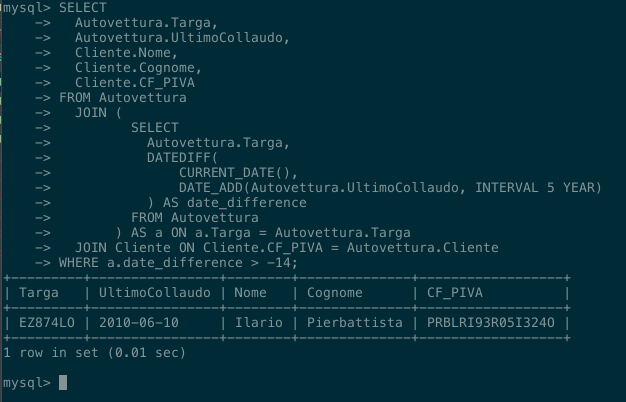
\includegraphics[width=9cm]{images/screenshots/list_collaudo_scadenza.png}
              \end{figure}


            \item[\ref{op:show_revisione}] Consultazione della data di ultima revisione per un'autovettura.
              \begin{lstlisting}
SELECT UltimaRevisione
FROM Autovettura
WHERE Targa = <Targa dell'autovettura>;
              \end{lstlisting}

              Analogamente al caso precedente è utile avere una lista delle autovetture la cui scadenza della revisione è prossima. Vista la forte analogia con il caso precedente, non riportiamo alcuno screenshot.
              \begin{lstlisting}
/** Lista delle autovetture (con relativi proprietari)
 *  che necessitano di una nuova revisione entro 14 giorni.
 */
SELECT
  Autovettura.Targa,
  Autovettura.UltimaRevisione,
  Cliente.Nome,
  Cliente.Cognome,
  Cliente.CF_PIVA
FROM Autovettura
  JOIN (
         SELECT
           Autovettura.Targa,
           DATEDIFF(
               CURRENT_DATE(),
               DATE_ADD(Autovettura.UltimaRevisione, INTERVAL 5 YEAR)
           ) AS date_difference
         FROM Autovettura
       ) AS a ON a.Targa = Autovettura.Targa
  JOIN Cliente ON Cliente.CF_PIVA = Autovettura.Cliente
WHERE a.date_difference > -14;
              \end{lstlisting}

            \item[\ref{op:show_fattura}] La visualizzazione dei dati di una fattura si articola in due fasi. La prima fase prevedere l'estrazione dei dati per stilare l'intestazione della fattura e la parte relativa agli importi.

            Ogni fattura nella sezione dedicata agli importi dovrà contenere l'\emph{imponibile Lordo}, lo \emph{sconto} in percentuale, l'\emph{Importo dello sconto}, l'\emph{imponibile netto}, l'ammontare delle \emph{imposte}, il valore di eventuali \emph{incentivi}, il \emph{totale}, il valore di un eventuale \emph{acconto} e il \emph{totale al netto dell'acconto}.

            Disponiamo solamente dell'\emph{imponibile netto} (attributo \emph{Imponibile} di \emph{Fattura}), del valore percentuale dello \emph{sconto} (attributo \emph{Sconto} di \emph{Fattura}), del valore degli \emph{incentivi} (attributo \emph{Incentivi} di \emph{Fattura}) e del valore dell'\emph{acconto} (attributo \emph{Quota} di \emph{Transazione}).

            Siano $i$, $s$, $A$, $D$, rispettivamente l'\emph{imponibile netto}, lo \emph{sconto percetuale}, l'\emph{acconto}, gli \emph{incentivi}. Sia inoltre $IVA$ l'ammontare in percentuale dell'iva.

            Sia $I$ l'\emph{imponibile lordo}, l'equazione \ref{eq:imponibile_lordo} fornisce la relazione con i parametri conosciuti.
            \begin{equation}
              \label{eq:imponibile_lordo}
              i = (1 - \frac{s}{100})\cdot I \Rightarrow I = \frac{i}{1 - \frac{s}{100}} \\
              \Rightarrow I = \frac{100 \cdot i}{100 - s} 
            \end{equation}

            Sia $S$ l'\emph{importo dello sconto}:
            \begin{equation}
              \label{eq:importo_sconto}
              I = i + S \Rightarrow S = i\cdot \left( \frac{100}{100 - s} - 1 \right) \\
              \Rightarrow S = i \cdot \left( \frac{s}{100 - s} \right)
            \end{equation}

            Sia $T$ il valore delle imposte:
            \begin{equation}
              \label{eq:imposte}
              T = i \cdot \frac{IVA}{100}
            \end{equation}

            Sia $TOT$ il \emph{totale lordo}:
            \begin{equation}
              \label{eq:totale_lordo}
              TOT = i + T - D
            \end{equation}

            Sia $tot$ il \emph{totale netto}:
            \begin{equation}
              \label{eq:totale_netto}
              tot = TOT - A
            \end{equation}

            Si assume che l'iva sia al $22\%$.

              \begin{lstlisting}
SELECT
  Fattura.Numero,
  Fattura.Anno,
  Fattura.DataEmissione,
  Fattura.SisPag,
  Cliente.Nome,
  Cliente.Cognome,
  Cliente.Citta,
  Cliente.Via,
  Cliente.Civico,
  Cliente.CAP,
  Autovettura.Targa,
  f.ImponibileLordo,
  Fattura.Sconto,
  f.ImportoSconto,
  Fattura.Imponibile                                    AS ImponibileNetto,
  f.Imposte,
  Fattura.Incentivi,
  Fattura.Imponibile + f.Imposte - Fattura.Incentivi    AS Totale,
  IFNULL(Transazione.Quota, 0)                          AS RitenutaAcconto,
  Fattura.Imponibile + f.Imposte - 
      Fattura.Incentivi - IFNULL(Transazione.Quota, 0)  AS TotaleNetto
FROM Fattura
  JOIN Preventivo ON Preventivo.Codice = Fattura.Prestazione
  LEFT JOIN Transazione ON Transazione.Codice = Preventivo.Acconto
  JOIN Autovettura ON Autovettura.Targa = Preventivo.Autovettura
  JOIN Cliente ON Cliente.CF_PIVA = Autovettura.Cliente
  JOIN (SELECT
          Fattura.Numero,
          Fattura.Anno,
          ROUND(Fattura.Imponibile * (100 / (100 - Fattura.Sconto)), 2)
            AS ImponibileLordo,
          ROUND(Fattura.Imponibile * 0.22, 2)                                      
            AS Imposte,
          ROUND(Fattura.Imponibile * (Fattura.Sconto / (100 - Fattura.Sconto)), 2) 
            AS ImportoSconto
        FROM Fattura) AS f ON Fattura.Numero = f.Numero AND Fattura.Anno = f.Anno;
              \end{lstlisting}

          \end{description}
